\section{Results}
\label{sec:results}
% Give the outcomes for each research question in the form of a table or graphic (with caption).
% Write about your results here. Good captions to tables and/or figures are key.

\subsection{Transformer models}

The training curves during the pretraining stage of the transformer models is shown in Figure~\ref{fig:pretain_loss_curve}. For reference, the original U-Net model also undergoing the same pretraining process is shown for comparison. The expected loss from an untrained classifier ($2k\log_e2$) is subtracted from the binary-cross entropy loss. The initial loss of the network is thus close to zero. From this graph, we can conclude firstly that the MTS network performs relatively poorly, and since it will not be competitive with the ViT or U-Net models, we chose to not use it any further. 

\begin{figure}[htb]
  \centering
  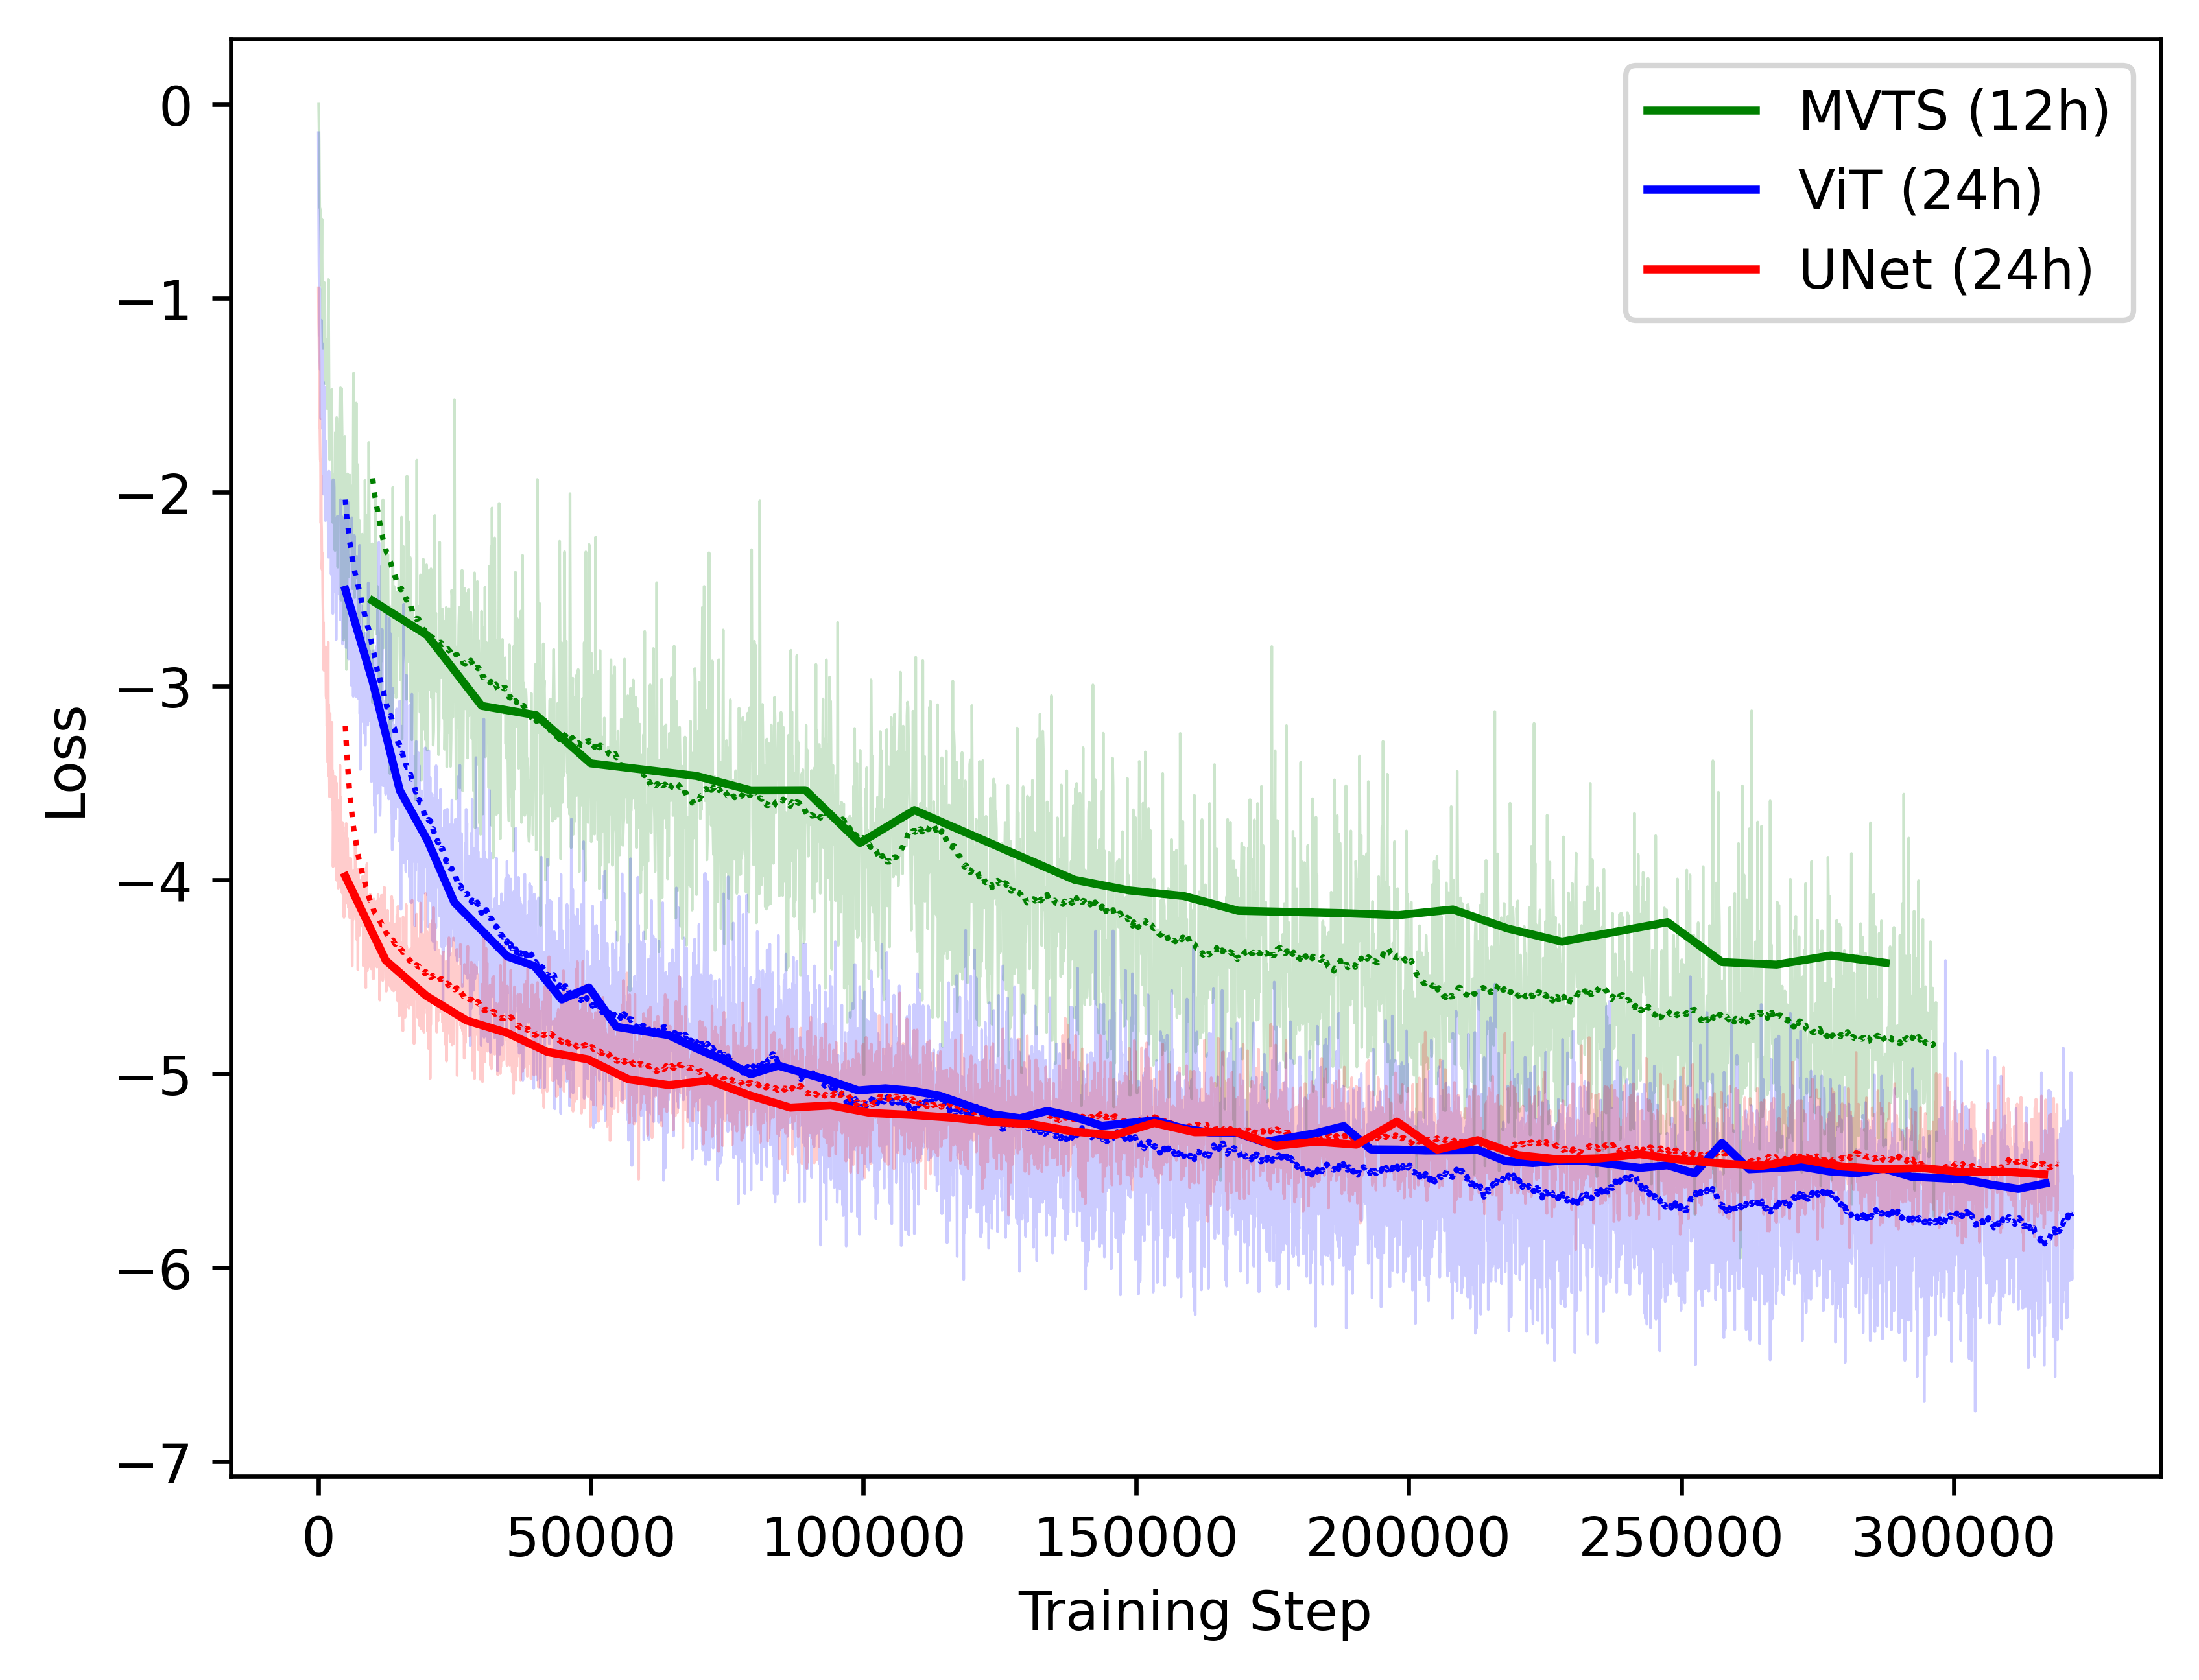
\includegraphics[width=1\linewidth]{media/images/Pretraining_loss_curve.png}
  \caption{Training curves for the two transformer models and U-Net. The original training loss is shown in transparent, the smoothed average (period 50) of the training loss is shown in dotted lines, and the validation loss is shown as a solid line.}
  \Description[<short description>]{<long description>}
  \label{fig:pretain_loss_curve}
\end{figure}

The validation loss of the U-Net and ViT converges to very similar values, so the ViT model does not seem to extract any information above and beyond the U-Net model. In Table~\ref{tab:loss_pretraining}, the loss per parameter at the end of the pretraining is given. 

\begin{table}[htb]
    \caption{Loss values for each of the parameters}
    \label{tab:loss_pretraining}
    \begin{tabular}{lrrr}
    \toprule
    Parameter & MTS & ViT & U-Net \\
    \midrule
    \textit{Intrinsic} &&& \\
    $q$ & -0.231 & -0.295 & -0.300 \\
    $M$ & -0.542 & -0.676 & -0.701 \\
    $\theta_{jn}$ & -0.327 & -0.463 & -0.426 \\
    $\phi_c$ & 0.000 & 0.000 & 0.000 \\
    $\theta_1$ & -0.107 & -0.167 & -0.174 \\
    $\theta_2$ & -0.018 & -0.036 & -0.036 \\
    $a_1$ & -0.078 & -0.104 & -0.132 \\
    $a_2$ & -0.005 & -0.008 & -0.007 \\
    $\phi_{12}$ & 0.000 & 0.000 & 0.000 \\
    $\phi_{jl}$ & -0.199 & -0.291 & -0.287 \\
    \midrule
    \textit{Extrinsic} &&& \\
    $d_L$ & -0.196 & -0.294 & -0.291 \\
    $\delta$ & -0.830 & -0.923 & -0.899 \\
    $\alpha$ & -1.020 & -1.085 & -1.066 \\
    $\psi$ & -0.063 & -0.117 & -0.090 \\
    $t_c$ & -0.965 & -1.104 & -1.105 \\
    \bottomrule
    \end{tabular}
\end{table}

\subsection{Peregrine Networks}

The results of the different networks integrated into \texttt{peregrine} is shown in Table~\ref{tab:peregrine_network_results}. In addition to the change in network architectures, we also include two additional cases, \enquote{U-Net (half)} and \enquote{U-Net (NR)}. The \enquote{U-Net (half)} is the \enquote{U-Net} with half the number of simulations per round (refer back to Table~\ref{tab:default_run_settings}) and the \enquote{NR} in \enquote{U-Net (NR)} stands for \enquote{No Re-initialization}. In the original \texttt{peregrine}, each simulation round begins with a freshly initialised network i.e. the weights are set back to random. For the \enquote{NR} case, we transfer the weights of the trained network to the following round. The number of training steps can be used as a measure of time to train the network each round. For the U-Net architectures, the batch size is 256, while for ViT it was 64. However, each training step takes approximately the same amount of time.

\begin{table}[htb]
\caption{Network performance of different network architectures for Peregrine. The first U-Net is the performance baseline.}
\label{tab:peregrine_network_results}
\hspace{-0.0cm}
\adjustbox{max width=1.0\columnwidth}{
\begin{tabular}{@{}lrrrrrrr@{}}
\toprule
\multicolumn{1}{@{}p{0.5cm}@{}}{\raggedright Network}  & 
\multicolumn{1}{@{}p{0.5cm}@{}}{\raggedright Rnd}  &
\multicolumn{1}{@{}p{1cm}@{}}{\raggedleft Num \\ Epochs} &
\multicolumn{1}{@{}p{1cm}@{}}{\raggedleft Num \\ Steps} &
\multicolumn{1}{@{}p{1cm}@{}}{\raggedleft Trunc \\ Fraction} &
\multicolumn{1}{@{}p{0.75cm}@{}}{\raggedleft Train \\ Loss} &
\multicolumn{1}{@{}p{0.75cm}@{}}{\raggedleft Test \\ Loss} &
\multicolumn{1}{@{}p{1cm}@{}}{\raggedleft Avg \\ AUROC} \\
\midrule
U-Net & 1 & 57 & 5757 & 4.47e-02 & -4.00 & -4.03 & 0.701 \\
U-Net & 2 & 115 & 23920 & 2.04e-04 & -4.49 & -4.24 & 0.718 \\
U-Net & 3 & 80 & 24720 & 6.33e-06 & -4.57 & -4.71 & 0.743 \\
U-Net & 4 & 70 & 29190 & 2.13e-06 & -4.71 & -4.61 & 0.747 \\
U-Net & 5 & 44 & 18348 & 1.61e-06 & -4.09 & -4.10 & 0.735 \\
U-Net & 6 & 80 & 41920 & 9.33e-07 & -4.39 & -4.39 & 0.742 \\
U-Net & 7 & 45 & 23580 & 9.29e-07 & -4.68 & -4.33 & 0.739 \\
U-Net & 8 & 108 & 56592 & 7.29e-07 & -4.76 & -4.54 & 0.746 \\
\midrule
U-Net (half) & 1 & 94 & 4606 & 3.67e-02 & -4.74 & -3.95 & 0.706 \\
U-Net (half) & 2 & 83 & 8383 & 1.10e-02 & -3.82 & -3.48 & 0.698 \\
U-Net (half) & 3 & 78 & 12246 & 9.88e-04 & -3.70 & -3.66 & 0.706 \\
U-Net (half) & 4 & 84 & 17472 & 7.67e-06 & -4.56 & -4.62 & 0.738 \\
U-Net (half) & 5 & 58 & 12064 & 3.80e-06 & -4.29 & -4.25 & 0.735 \\
U-Net (half) & 6 & 60 & 15840 & 2.36e-06 & -4.10 & -4.30 & 0.741 \\
U-Net (half) & 7 & 68 & 17952 & 1.75e-06 & -4.06 & -4.12 & 0.734 \\
U-Net (half) & 8 & 69 & 18216 & 1.16e-06 & -4.35 & -4.20 & 0.735 \\
\midrule
U-Net (NR) & 1 & 61 & 6161 & 4.99e-02 & -4.36 & -3.98 & 0.700 \\
U-Net (NR) & 2 & 55 & 11440 & 1.64e-03 & -4.30 & -4.03 & 0.709 \\
U-Net (NR) & 3 & 65 & 20085 & 1.24e-05 & -4.68 & -4.59 & 0.734 \\
U-Net (NR) & 4 & 52 & 21684 & 1.95e-06 & -5.01 & -4.78 & 0.750 \\
U-Net (NR) & 5 & 46 & 19182 & 1.12e-06 & -4.42 & -4.32 & 0.740 \\
U-Net (NR) & 6 & 38 & 19912 & 8.91e-07 & -4.77 & -4.45 & 0.743 \\
U-Net (NR) & 7 & 56 & 29344 & 7.01e-07 & -4.34 & -4.48 & 0.741 \\
U-Net (NR) & 8 & 30 & 15720 & 6.87e-07 & -4.49 & -4.47 & 0.743 \\
\midrule
Att U-Net & 1 & 70 & 7070 & 3.07e-03 & -4.67 & -4.23 & 0.707 \\
Att U-Net & 2 & 108 & 22464 & 1.18e-05 & -4.79 & -4.83 & 0.742 \\
Att U-Net & 3 & 67 & 20703 & 7.70e-06 & -4.59 & -4.32 & 0.737 \\
Att U-Net & 4 & 82 & 34194 & 4.98e-06 & -4.42 & -4.36 & 0.739 \\
Att U-Net & 5 & 61 & 25437 & 4.25e-06 & -4.52 & -4.46 & 0.743 \\
Att U-Net & 6 & 70 & 36680 & 2.63e-06 & -4.06 & -4.43 & 0.741 \\
Att U-Net & 7 & 56 & 29344 & 2.61e-06 & -4.50 & -4.41 & 0.740 \\
Att U-Net & 8 & 58 & 30392 & 2.57e-06 & -4.56 & -4.40 & 0.741 \\
\midrule
U-Net 5\% & 1 & 31 & 3131 & 1.57e-02 & -4.52 & -3.93 & 0.685 \\
U-Net 5\% & 2 & 30 & 6240 & 2.31e-04 & -4.73 & -4.19 & 0.713 \\
U-Net 5\% & 3 & 68 & 21012 & 8.50e-06 & -4.57 & -4.56 & 0.743 \\
U-Net 5\% & 4 & 48 & 20016 & 2.10e-06 & -5.06 & -4.63 & 0.748 \\
U-Net 5\% & 5 & 47 & 19599 & 1.49e-06 & -4.57 & -4.38 & 0.742 \\
U-Net 5\% & 6 & 48 & 25152 & 1.34e-06 & -4.40 & -4.53 & 0.743 \\
U-Net 5\% & 7 & 30 & 15720 & 1.19e-06 & -4.23 & -4.28 & 0.739 \\
U-Net 5\% & 8 & 89 & 46636 & 8.64e-07 & -4.65 & -4.52 & 0.745 \\
\midrule
U-Net 10\% & 1 & 39 & 3939 & 4.31e-02 & -3.98 & -3.89 & 0.689 \\
U-Net 10\% & 2 & 35 & 7280 & 3.72e-03 & -3.67 & -3.76 & 0.706 \\
U-Net 10\% & 3 & 58 & 17922 & 4.33e-05 & -4.42 & -4.62 & 0.732 \\
U-Net 10\% & 4 & 57 & 23769 & 1.14e-05 & -4.54 & -4.27 & 0.735 \\
U-Net 10\% & 5 & 30 & 12510 & 8.17e-06 & -3.90 & -3.96 & 0.725 \\
U-Net 10\% & 6 & 56 & 29344 & 4.87e-06 & -4.08 & -4.31 & 0.738 \\
U-Net 10\% & 7 & 73 & 38252 & 3.23e-06 & -4.22 & -4.26 & 0.738 \\
U-Net 10\% & 8 & 43 & 22532 & 3.07e-06 & -4.17 & -4.11 & 0.734 \\
\midrule
ViT & 1 & 30 & 12540 & 9.68e-05 & -6.27 & -5.72 & 0.750 \\
ViT & 2 & 38 & 31958 & 4.71e-06 & -5.66 & -5.07 & 0.759 \\
ViT & 3 & 40 & 50360 & 2.39e-06 & -4.91 & -4.61 & 0.750 \\

\bottomrule
\end{tabular}}
\end{table}


Due to the very slow progress of the ViT model, it was stopped after only completing three rounds to save some computer budget. In terms of training times/steps of the other networks, the run with half the number of training samples took about 50\% of the time to train compared to the baseline case. The U-Net that was not reinitialized finished the runs about 35\% faster, the attention U-Net was 8\% faster, the U-Net pruned models were both 30\% faster. Although the U-Net 10\% pruned model took faster to train, we can also see that the loss values were higher than the other cases, suggesting that the network started to drop in performance.

For all the different networks the truncation rapidly decreases in the first four rounds before reducing only very slightly in the subsequent rounds. This means that after 5 rounds or so, the parameter range of interest has been identified, and the posteriors will start to be constructed with higher precision. The original U-Net and U-Net with no re-initialisation is able to reduce the parameter space most efficiently. 

Table~\ref{tab:peregrine_network_results} shows a summary of performance metrics for the different networks. However, we still cannot conclude the best option without comparing the posterior plots. The posterior plots are given in Figures~\ref{fig:posterior_unet_half}--\ref{fig:posterior_vit} in the appendix.

%\FloatBarrier

%\begin{table}[htb]
%\caption{AUROC curve for all parameters calculated at the end of round 7.}
%\hspace*{0cm}
%\begin{tabular}{lrrrrr}
%\toprule
%Param & 
%\multicolumn{1}{p{0.3cm}}{\raggedright UNet}  & 
%\multicolumn{1}{p{0.3cm}}{\raggedleft UNet (NR)}  &
%\multicolumn{1}{p{0.3cm}}{\raggedleft Att UNet}  &
%\multicolumn{1}{p{0.3cm}}{\raggedleft UNet 5\%}  &
%\multicolumn{1}{p{0.3cm}}{\raggedleft UNet 10\%}  \\
%\midrule
%$q$ & 0.782 & 0.786 & 0.780 & 0.773 & 0.733 \\
%$M$ & 0.822 & 0.828 & 0.820 & 0.825 & 0.818 \\
%$\theta_{jn}$ & 0.807 & 0.785 & 0.797 & 0.823 & 0.818 \\
%$\phi_c$ & 0.496 & 0.501 & 0.497 & 0.493 & 0.500 \\
%$\theta_1$ & 0.761 & 0.767 & 0.755 & 0.758 & 0.751 \\
%$\theta_2$ & 0.643 & 0.639 & 0.636 & 0.636 & 0.633 \\
%$a_1$ & 0.731 & 0.734 & 0.723 & 0.730 & 0.715 \\
%$a_2$ & 0.574 & 0.574 & 0.574 & 0.574 & 0.567 \\
%$\phi_{12}$ & 0.498 & 0.493 & 0.493 & 0.501 & 0.503 \\
%$\phi_{jl}$ & 0.867 & 0.910 & 0.902 & 0.903 & 0.891 \\
%$d_L$ & 0.825 & 0.816 & 0.814 & 0.824 & 0.816 \\
%$\delta$ & 0.850 & 0.848 & 0.858 & 0.855 & 0.854 \\
%$\alpha$ & 0.859 & 0.857 & 0.864 & 0.857 & 0.858 \\
%$\psi$ & 0.725 & 0.718 & 0.722 & 0.753 & 0.747 \\
%$t_c$ & 0.852 & 0.859 & 0.867 & 0.861 & 0.857 \\
%\bottomrule
%\end{tabular}
%\end{table}

%\subsection{Peregrine Run Strategy}

%In this section we show the results of varying the number of simulations, and the different sampling strategies.

% Network reinitialisation

% 
% Sampling strategy
% Simulation scheduling

% Compare posteriors of 

% Sometimes,  especially  if  you  have  quite  different experiments or research  questions,  it makes sense to interleave the experimental setup and the results sections, so the reader does not get lost. It is then helpful to structure clearly in (sub)subsections.